\documentclass[tikz,border=5pt]{standalone}
\usepackage{tikz}
\usetikzlibrary{arrows.meta}
\begin{document}
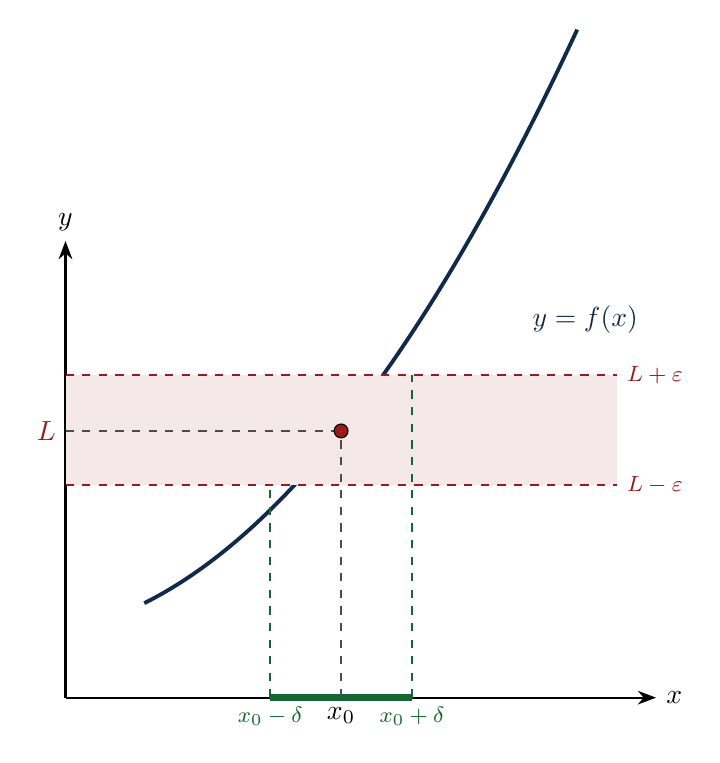
\begin{tikzpicture}[>=Stealth, scale=1.0]
  \definecolor{navyblue}{HTML}{0F2A4A}
  \definecolor{setblue}{HTML}{1E40AF}
  \definecolor{accentcrimson}{HTML}{991B1B}
  \definecolor{forestgreen}{HTML}{166534}

  % Axes
  \draw[thick, ->] (0,0) -- (7.5,0) node[right, font=\sffamily\bfseries] {$x$};
  \draw[thick, ->] (0,0) -- (0,5.8) node[above, font=\sffamily\bfseries] {$y$};

  % Function curve
  \draw[line width=1.4pt, navyblue, domain=1.0:6.5, samples=100] 
    plot (\x, {1.2 + 0.5*(\x - 1) + 0.15*(\x - 1)*(\x - 1)});
  \node[navyblue, font=\sffamily\bfseries] at (6.6, 4.8) {$y = f(x)$};

  % Coordinates x0, L
  \coordinate (X0) at (3.5, 0);
  \coordinate (P) at (3.5, {1.2 + 0.5*(2.5) + 0.15*(6.25)}); % ~3.3875
  \coordinate (L) at (0, 3.3875);

  % Epsilon tube on y-axis
  \fill[accentcrimson!10] (0, 2.7) rectangle (7.0, 4.1);
  \draw[thick, dashed, accentcrimson] (0, 4.1) -- (7.0, 4.1) node[right, font=\sffamily\footnotesize] {$L + \varepsilon$};
  \draw[thick, dashed, accentcrimson] (0, 2.7) -- (7.0, 2.7) node[right, font=\sffamily\footnotesize] {$L - \varepsilon$};
  \draw[thick, dashed, black!70] (0, 3.3875) -- (3.5, 3.3875);
  \node[left, accentcrimson, font=\sffamily\bfseries] at (0, 3.3875) {$L$};

  % Delta interval on x-axis
  \draw[line width=2.5pt, forestgreen] (2.6, 0) -- (4.4, 0);
  \draw[thick, dashed, forestgreen] (2.6, 0) -- (2.6, 2.7);
  \draw[thick, dashed, forestgreen] (4.4, 0) -- (4.4, 4.1);
  \node[below, font=\sffamily\bfseries] at (3.5, 0) {$x_0$};
  \node[below, forestgreen, font=\sffamily\footnotesize] at (2.6, 0) {$x_0 - \delta$};
  \node[below, forestgreen, font=\sffamily\footnotesize] at (4.4, 0) {$x_0 + \delta$};

  \draw[fill=accentcrimson] (P) circle (2.5pt);
  \draw[thick, dashed, black!70] (3.5, 0) -- (P);
\end{tikzpicture}
\end{document}